% !TeX program = pdflatex
% !TeX spellcheck = en_US
% !TeX encoding = UTF-8

% update
% v.1.2 - 2018-10-15
% - Felix: use Bibtex instead of Biblatex
% v1.10 - 2017-05-30
% - Erik: Refactor the file structure of the front pages
% - Erik: Fix double bibliography entry
% v1.9 - 2017-02-03
% - Dirk: fixed warning: Underfull \hbox (badness 10000) in paragraph main.tex
% - Dirk: fixed warning: "Data encoding is UTF8" -> style.tex 0.1.8
% v1.8 - 2017-02-02
% - Dirk: replaced titlesec package by KOMA-script commands.-> style.tex v0.1.7
% v1.7 - 2014-11-18
% - bib fixes: now using biber instead of bibtex (thanks felix)
% - compile now with pdflatex -> biber -> pdflatex
% v1.6 - 2013-05-13
% - bibliography headers fixed - thanx lorenz lehmann
% - high quality titlepage - thanx thomas graf
% - removed separation of online and offline references -> style 1.4a
% v1.5 - 2013-01-16

\documentclass[twoside,11pt,titlepage,a4paper,english,bibliography=totocnumbered,listof=numbered]{scrbook}
%
% Template Style
% =========================================================================
% = SNET THESIS TEMPLATE STYLE
% =========================================================================

% http://www.snet.tu-berlin.de
% ------------------------
% Adapted version from http://hci.rwth-aachen.de/karrer_thesistemplate (Thorsten Karrer)
% Further adaptions for http://www.elearn.rwth-aachen.de (Sascha Hoellger)
% Further adaptions for SNET @ TU Berlin by Sebastian Göndör (sebastian.goendoer@tu-berlin.de)


% =========================================================================
% = CHANGELOG
% =========================================================================
% [0.1.9]
% - Fixed styling for chapters and toc using Komascript
% - Remove double bibliography TOC entry
%
% [0.1.8]
% - fixed "warning UFT8 is used". biblatex requires ascii encoding; by Dirk
%
% [0.1.7]
% replaced "Titelsec" commands (and whole package) by appropriate KOMA-Script commands; by Dirk
%
% [0.1.6]
% replaced deprecated \rm commands with \rmfamily commands; by Dirk
%
% [0.1.4b]
% backend=biber added in line 139
%
% [0.1.4a]
% title page: image logo sizes and margins adjusted to printable area
% removed separation of online and offline references
%
% [0.1.3]
% wider text body
% added "school" to the titlepage
% paragraph indents
% correctly placed footnote graphics
%
% [0.1.2]
% new titlepage
% some minor fixes
%
% [0.1.1]
% changed titlepage logo
% added listoffigures and listoftables
% excluded abstract from toc
% no (roman) numbering for frontmatter
%
% [0.1]
% adapted version 0.991b from sascha hoellger @ rwth aachen


% =========================================================================
% = MISC
% =========================================================================

\usepackage{a4wide}					%
\usepackage{verbatim}				%
\usepackage[toc,page]{appendix}			%
\usepackage[withpage]{acronym}			%
\usepackage{amsthm}				% Definitions


% =========================================================================
% = COLORS
% =========================================================================

\usepackage{xcolor}					% Colors
\definecolor{LightBlue}{rgb}{0.55,0.55,1}
\definecolor{DarkBlue}{rgb}{0.2,0.2,0.5}
\definecolor{DarkRed}{rgb}{0.71,0.12,0.07}

% =========================================================================
% = PAGE LAYOUT
% =========================================================================

\usepackage{geometry}
\geometry{inner=3cm, outer=2cm, bottom=4cm}

\newcommand{\setwidesite}				% changes the geometry to have less margin
{
	\fancyhfoffset[LE,RO]{0cm}
	\fancyheadoffset[LO,RE]{0cm}
	\fancyfootoffset[RE]{2cm}
	\newgeometry{inner=2cm, outer=2cm, bottom=4cm}
}

\usepackage{style/noindent}				%do not indent at new paragraphs but add a vertical offset

\setlength{\parindent}{4mm}
\setlength{\parskip}{1.5mm }


% =========================================================================
% = TYPESETTING
% =========================================================================

\usepackage[hyphens]{url}				% url
\usepackage{hyphenat}				% hyphenation. use \hyphenation{}

\righthyphenmin=5
\lefthyphenmin=5


% =========================================================================
% = TABLE OF CONTENTS
% =========================================================================

\setcounter{secnumdepth}{4}
\setcounter{tocdepth}{3}

\addtokomafont{disposition}{\rmfamily}


% =========================================================================
% = FONTS
% =========================================================================

\usepackage{mathpazo}
\usepackage[scaled=.95]{helvet}
\usepackage{courier}


% =========================================================================
% = SYMBOLS
% =========================================================================

%\usepackage{gensymb}
\usepackage{textcomp} 				% for \textmu (non-italic $\mu$)
\makeatletter						% this makes "@" a regular letter


% =========================================================================
% = TABLES
% =========================================================================

\usepackage{tabularx}
\usepackage{booktabs}
\usepackage{multirow}
\usepackage{longtable}				% tables spanning over more than one page

%%\setlength{\fboxsep}{0mm}			% spacing between \fbox border and content

\usepackage{amsmath}				% math fonts
\usepackage{amssymb}				% math symbols
\usepackage{setspace}				% line spacing


% =========================================================================
% = BIBILOGRAPHY
% =========================================================================

% 2018-10-16 - changed to use Bibtex instead

%\usepackage[style=numeric,natbib=true,backend=biber]{biblatex}

% apparently no effect?
%\renewcommand{\bibsetup}{
%	\markboth{
%		\MakeUppercase{Bibliography}
%	}{}
%}

%\ifdefined\bibheadingonline
%  \defbibheading{online}{\section*{\bibheadingonline}}
%\else
%  \defbibheading{online}{\section*{Online References}}
%\fi
%\ifdefined\bibheadingoffline
%  \defbibheading{offline}{\section*{\bibheadingoffline}}
%\else
%  \defbibheading{offline}{\section*{Printed References}}
%\fi
%
%\defbibfilter{online}{%
%  \( \type{online} \)}
%
%\defbibfilter{offline}{%
%  \( \not \type{online} \)}
%
%\bibliography{Bibliography}


% =========================================================================
% = LANGUAGE & ENCODING
% =========================================================================

\usepackage[english]{babel}				% \usepackage[ngerman]{babel}

\selectlanguage{english}				% \selectlanguage{ngerman}

\usepackage[T1]{fontenc}
\usepackage[utf8]{inputenc}				% can use native umlauts

% \usepackage[babel,german=quotes]{csquotes}	% provides \enquote{Blupp} => "`Blupp"'
\usepackage[babel,english=american]{csquotes}	% provides \enquote{Blupp} => "`Blupp"'

%\SetCiteCommand{\parencite}			% Changed for biblatex

\usepackage{units}					% unified way of setting values with units

\usepackage{appendix}


% =========================================================================
% = CODE LISTINGS
% =========================================================================

\usepackage{listings}

% Listings Styles from Max

\definecolor{violet}{cmyk}{0.45,0.97,0.27,0.21}
\definecolor{lstblue}{cmyk}{1,0.80,0,0}
\definecolor{lstgreen}{cmyk}{0.71,0.21,0.65,0.22}
\definecolor{bluegrey}{cmyk}{0.56,0.24,0.11,0.05}
\definecolor{javadoc}{cmyk}{0.88,0.59,0,0}
\definecolor{lstgrey}{cmyk}{0.55,0.44,0.42,0.32}

\lstdefinelanguage{SQL}{
     keywords={},
     keywordstyle=\color{bluegrey}\bfseries,
     morekeywords=[2]{CREATE,TABLE,IF,NOT,EXISTS,NULL,SET,DEFAULT,PRIMARY,KEY,COLLATE,CHARACTER,AUTO_INCREMENT,ENGINE,CHARSET},
     keywordstyle={[2]\color{violet}\bfseries},
     otherkeywords={int,varchar,double,text,tinyint},
     sensitive=false,
     morecomment=[l][\color{lstgreen}]{//},
     morecomment=[s][\color{lstgreen}]{/*}{*/},
     morecomment=[s][\color{javadoc}]{/**}{*/},
     morestring=[b]',
     morestring=[b]"
  }
\lstdefinelanguage{PHP}{
     keywords={},
     keywordstyle=\color{bluegrey}\bfseries,
     morekeywords=[2]{static,function,if,return,pow,sin,cos,asin,min,sqrt,int},
     keywordstyle={[2]\color{violet}\bfseries},
     otherkeywords={@param, @returns, @author, @type, @link, @see},
     sensitive=false,
     morecomment=[l][\color{lstgreen}]{//},
     morecomment=[s][\color{lstgreen}]{/*}{*/},
     morecomment=[s][\color{javadoc}]{/**}{*/},
     morestring=[b]',
     morestring=[b]"
  }
\lstdefinelanguage{JavaScript}{
     keywords={},
     keywordstyle=\color{bluegrey}\bfseries,
     morekeywords=[2]{attributes, class, classend, do, empty, endif, endwhile, fail, function, functionend, if, implements, in, inherit, inout, not, of, operations, out, return, set, then, types, while, use},
     keywordstyle={[2]\color{violet}\bfseries},
     otherkeywords={@param, @returns, @author, @type, @link, @see},
     sensitive=false,
     morecomment=[l][\color{lstgreen}]{//},
     morecomment=[s][\color{lstgreen}]{/*}{*/},
     morecomment=[s][\color{javadoc}]{/**}{*/},
     morestring=[b]',
     morestring=[b]"
  }
\lstdefinelanguage{Java}{
     keywords={},
     keywordstyle=\color{bluegrey}\bfseries,
     morekeywords=[2]{abstract,boolean,break,byte,case,catch,char,class,
      const,continue,default,do,double,else,extends,false,final,
      finally,float,for,goto,if,implements,import,instanceof,int,
      interface,label,long,native,new,null,package,private,protected,
      public,return,short,static,super,switch,synchronized,this,throw,
      throws,transient,true,try,void,volatile,while},
     keywordstyle={[2]\color{violet}\bfseries},
     morekeywords=[3]{@SuppressWarnings, @Capability, @Override},
     keywordstyle={[3]\color{lstgrey}},
     otherkeywords={@param, @return, @returns, @author, @link, @see},
     sensitive,
     morecomment=[l]//,
     morecomment=[s]{/*}{*/},
     morecomment=[s][\color{javadoc}]{/**}{*/},
     morestring=[b]",
     morestring=[b]',
  }[keywords,comments,strings]

% some listings styles from Gregor Aisch
% http://vis4.net/blog/2009/09/noch-mehr-sprach-definitionen-fuer-latex-listings/

\lstdefinelanguage{HTML5} {morekeywords={a, abbr, address, area, article, aside, audio, b, base, bb, bdo, blockquote,  body, br, button, canvas, caption, cite, code, col, colgroup, command, datagrid, datalist, dd, del, details, dialog, dfn, div, dl, dt, em, embed, eventsource, fieldset, figure, footer,  form,  h1, h2,  h3,  h4, h5,  h6,  head,  header,  hr, html,  i, iframe,  img,  input,  ins, kbd,  label,  legend,  li,  link,  mark,  map,  menu,  meta,  meter,  nav,  noscript,  object,  ol,  optgroup,  option,  output,  p,  param,  pre,  progress,  q,  ruby,  rp,  rt,  samp,  script,  section,  select,  small,  source,  span,  strong,  style,  sub,  sup,  table,  tbody,  td,  textarea,  tfoot,  th,  thead,  time,  title,  tr,  ul,  var,  video},
sensitive=false, morecomment=[s]{<!--}{-->}, morestring=[b]", morestring=[d]'}

\lstdefinelanguage{CSS} {morekeywords={azimuth,  background-attachment,  background-color,  background-image,  background-position,  background-repeat,  background,  border-collapse,  border-color,  border-spacing,  border-style,  border-top, border-right, border-bottom, border-left,  border-top-color, border-right-color, border-bottom-color, border-left-color,  border-top-style, border-right-style, border-bottom-style, border-left-style,  border-top-width, border-right-width, border-bottom-width, border-left-width,  border-width,  border,  bottom,  caption-side,  clear,  clip,  color,  content,  counter-increment,  counter-reset,  cue-after,  cue-before,  cue,  cursor,  direction,  display,  elevation,  empty-cells,  float,  font-family,  font-size,  font-style,  font-variant,  font-weight,  font,  height,  left,  letter-spacing,  line-height,  list-style-image,  list-style-position,  list-style-type,  list-style,  margin-right, margin-left,  margin-top, margin-bottom,  margin,  max-height,  max-width,  min-height,  min-width,  orphans,  outline-color,  outline-style,  outline-width,  outline,  overflow,  padding-top, padding-right, padding-bottom, padding-left,  padding,  page-break-after,  page-break-before,  page-break-inside,  pause-after,  pause-before,  pause,  pitch-range,  pitch,  play-during,  position,  quotes,  richness,  right,  speak-header,  speak-numeral,  speak-punctuation,  speak,  speech-rate,  stress,  table-layout,  text-align,  text-decoration,  text-indent,  text-transform,  top,  unicode-bidi,  vertical-align,  visibility,  voice-family,  volume,  white-space,  widows,  width,  word-spacing,  z-index},
sensitive=false, morecomment=[s]{/*}{*/}, morestring=[b]", morestring=[d]'}

\lstdefinelanguage{JavaFX} {morekeywords={abstract, after, and, as, assert, at, attribute, before, bind, bound, break, catch, class, continue, def, delete, else, exclusive, extends, false, finally, first, for, from, function, if, import, indexof, in, init, insert, instanceof, into, inverse, last, lazy, mixin, mod, new, not, null, on, or, override, package, postinit, private, protected, public-init, public, public-read, replace, return, reverse, sizeof, static, step, super, then, this, throw, trigger, true, try, tween, typeof, var, where, while, with },
sensitive=false, morecomment=[l]{//}, morecomment=[s]{/*}{*/}, morestring=[b]", morestring=[d]'}

\lstdefinelanguage{MXML} {morekeywords={mx:Accordion, mx:Box, mx:Canvas, mx:ControlBar, mx:DividedBox, mx:Form, mx:FormHeading, mx:FormItem, mx:Grid, mx:GridItem, mx:GridRow, mx:HBox, mx:HDividedBox, mx:LinkBar, mx:Panel, mx:TabBar, mx:TabNavigator, mx:Tile, mx:TitleWindow, mx:VBox, mx:VDividedBox, mx:ViewStack, mx:Button, mx:CheckBox, mx:ComboBase, mx:ComboBox, mx:DataGrid, mx:DateChooser, mx:DateField, mx:HRule, mx:Image, mx:Label, mx:Link, mx:List, mx:Loader, mx:MediaController, mx:MediaDisplay, mx:MediaPlayback, mx:MenuBar, mx:NumericStepper, mx:ProgressBar, mx:RadioButton, mx:RadioButtonGroup, mx:Spacer, mx:Text, mx:TextArea, mx:TextInput, mx:Tree, mx:VRule, mx:VScrollBar, mx:Application, mx:Repeater, mx:UIComponent, mx:UIObject, mx:View, mx:FlexExtension, mx:UIComponentExtension, mx:UIObjectExtension, mx:Fade, mx:Move, mx:Parallel, mx:Pause, mx:Resize, mx:Sequence, mx:WipeDown, mx:WipeLeft, mx:WipeRight, mx:WipeUp, mx:Zoom, mx:EventDispatcher, mx:LowLevelEvents, mx:UIEventDispatcher, mx:CurrencyFormatter, mx:DateFormatter, mx:NumberFormatter, mx:PhoneFormatter, mx:ZipCodeFormatter, mx:CursorManager, mx:DepthManager, mx:DragManager, mx:FocusManager, mx:HistoryManager, mx:LayoutManager, mx:OverlappedWindows, mx:PopUpManager, mx:SystemManager, mx:TooltipManager, mx:CreditCardValidator, mx:DateValidator, mx:EmailValidator, mx:NumberValidator, mx:PhoneNumberValidator, mx:SocialSecurityValidator, mx:StringValidator, mx:ZipCodeValidator, mx:DownloadProgressBar, mx:ArrayUtil, mx:ClassUtil, mx:Delegate, mx:ObjectCopy, mx:URLUtil, mx:XMLUtil, mx:CSSSetStyle, mx:CSSStyleDeclaration, mx:CSSTextStyles, mx:StyleManager, mx:HTTPService, mx:RemoteObject, mx:Service},
sensitive=false, morecomment=[s]{<!--}{-->}, morestring=[b]", morestring=[d]'}

\lstdefinelanguage{LZX} {morekeywords={a, alert, animator, animatorgroup , attribute, audio , axis, axisstyle , b, barchart, basebutton , basebuttonrepeater , basecombobox , basecomponent , basedatacombobox , basedatepicker , basedatepickerday , basedatepickerweek , basefloatinglist , basefocusview , baseform , baseformitem , basegrid , basegridcolumn , baselist , baselistitem , basescrollarrow , basescrollbar , basescrollthumb , basescrolltrack , baseslider , basestyle , basetab , basetabelement , basetabpane , basetabs , basetabsbar , basetabscontent , basetabslider , basetrackgroup , basetree , basevaluecomponent , basewindow , br , button , canvas , chart , chartbgstyle , chartstyle , checkbox , class , columnchart , combobox , command , connection , connectiondatasource , constantboundslayout , constantlayout , datacolumn , datacombobox , datalabel , datamarker , datapath , datapointer , dataselectionmanager , dataseries , dataset , datasource , datastyle , datastylelist , datatip , datepicker , debug , dragstate , drawview , edittext , event , face , floatinglist , font , font , form , frame , grid , gridcolumn , gridtext , handler , hbox , horizontalaxis , hscrollbar , i , image , img , import , include , inputtext , javarpc , label , labelstyle , layout , legend , library , linechart , linestyle , list , listitem , LzTextFormat , menu , menubar , menuitem , menuseparator , method , modaldialog , multistatebutton , node , p , param , piechart , piechartplotarea , plainfloatinglist , plotstyle , pointstyle , pre , radiobutton , radiogroup , rectangularchart , regionstyle , remotecall , resizelayout , resizestate , resource , reverselayout , richinputtext , rpc , script , scrollbar , security , selectionmanager , sessionrpc , simpleboundslayout , simpleinputtext , simplelayout , slider , soap , splash , stableborderlayout , state , statictext , style , submit , swatchview , SyncTester , tab , tabelement , tabpane , tabs , tabsbar , tabscontent , tabslider , Test , TestCase , TestResult , TestSuite , text , textlistitem , tickstyle , tree , u , valueline , valuelinestyle , valuepoints , valuepointstyle , valueregion , valueregionstyle , vbox , verticalaxis , view , view , vscrollbar , webapprpc , window , windowpanel , wrappinglayout , XMLHttpRequest , xmlrpc , zoomarea},
sensitive=false, morecomment=[s]{<!--}{-->}, morestring=[b]", morestring=[d]'}

\lstset{
  numbers=left,
  numberstyle=\tiny,
  numbersep=5pt,
  breaklines=true,
  stepnumber=1,
  tabsize=2,
  basicstyle=\ttfamily\small,
  frame=none,
  numberfirstline=true,
  firstnumber=1,
  keywordstyle=\color{violet}\bfseries,
  ndkeywordstyle=\color{bluegrey}\bfseries,
  identifierstyle=\color{black},
  commentstyle=\color{lstgreen}\ttfamily,
  stringstyle=\color{lstblue}\ttfamily,
  showstringspaces=false
}


% ========================================================================
% = CHANGE LIST DEFINITIONS
% ========================================================================

% change color of item list
\renewcommand{\labelitemi}{\color{DarkRed}$\bullet$}
\renewcommand{\labelitemii}{\color{DarkRed}$\circ$}
\renewcommand{\labelitemiii}{\color{DarkRed}$\ast$}
\renewcommand{\labelitemiv}{\color{DarkRed}$\diamond$}

% change color of enum list
\renewcommand{\labelenumi}{\color{DarkRed}\arabic{enumi}.}
\renewcommand{\labelenumii}{\color{DarkRed}\alph{enumii})}
\renewcommand{\labelenumiii}{\color{DarkRed}\roman{enumiii}.}
\renewcommand{\labelenumiv}{\color{DarkRed}\Alph{enumiv}.}

% change color of description list
\usepackage{enumitem}
\setdescription{font=\color{DarkRed}\rmfamily\itshape}
% \renewenvironment{description}{\list{font=\color{DarkRed}\itshape}}{\endlist}


% ========================================================================
% = FOOTNOTES
% ========================================================================

% change color of footnotes
\renewcommand{\thefootnote}{\color{DarkRed}\arabic{footnote}}

% use nice footnote indentation
\deffootnote[1em]{1em}{1em}{\textsuperscript{\thefootnotemark}\,}


% =========================================================================
% = GRAPHICS AND IMAGES
% =========================================================================

\usepackage{graphicx}
\graphicspath{{images/}}				% path to your image folder

\usepackage{eso-pic}					% needed for the full-face titlepage
\usepackage{chngpage}				% we need this to determine if a figure is on an odd or even page
\usepackage{tikz}					% tikz pictures

% captions of tables and images
\usepackage[hang,small,sf]{caption}
\renewcommand{\captionfont}{\sffamily\small}
\renewcommand{\captionlabelfont}{\bfseries}

\usepackage{float}
\usepackage{placeins}
% \floatstyle{ruled}
%\floatplacement

\renewcommand{\floatpagefraction}{0.85}		% if a figure takes more than 85% of a page it will be typeset on a separate page
\usepackage[it,bf,tight,hang,raggedright]{subfigure}

%\numberwithin{figure}{section}
%\numberwithin{table}{section}


% =========================================================================
% = HEADER
% =========================================================================

\newcommand{\STYLEfootnotetext}
{
  \begin{minipage}
  {.2\textwidth}
    
\includegraphics[width=0.9\textwidth]{images/snet/snet_footer.png}
  \end{minipage}
}

% Change page headers and footers:
\usepackage{calc}
\usepackage{fancyhdr}
\pagestyle{fancy}
\fancyhfoffset[RO,LE]{0.1cm} %{\marginparsep+\marginparwidth}
\fancyhfoffset[RE,LO]{0.1cm}
%\fancyheadoffset[RE,LO]{\hoffset + \oddsidemargin}
\renewcommand{\headrule}{{\color{DarkRed}%
  \hrule width\headwidth height\headrulewidth \vskip-\headrulewidth}}
\fancyhf{}
\fancyhead[RE]{\slshape \nouppercase{\leftmark}}    % Even page header: "page   chapter"
\fancyhead[LO]{\slshape \nouppercase{\rightmark}}   % Odd  page header: "section   page"
\fancyhead[RO,LE]{\bfseries \thepage}

%- \fancyfoot[LE]{\STYLEleftpicture}
%- \fancyfoot[RO]{\STYLErightpicture}
\fancyfoot[LE]{\STYLEfootnotetext}

\renewcommand{\headrulewidth}{1pt}    % Underline headers
\renewcommand{\footrulewidth}{0pt}

% =========================================================================
% = SECTIONS THEMING
% =========================================================================

\newcommand{\allsectionformat}{\color{DarkRed}\rmfamily\normalfont}

% Font style and colors
\addtokomafont{part}{\Huge\allsectionformat}
\addtokomafont{chapter}{\Huge\allsectionformat}
\addtokomafont{section}{\allsectionformat}
\addtokomafont{subsection}{\allsectionformat}
\addtokomafont{subsubsection}{\allsectionformat}
\addtokomafont{paragraph}{\allsectionformat}
\addtokomafont{subparagraph}{\allsectionformat}

% Spacing before and after the section titles
\RedeclareSectionCommand[
  beforeskip=-.75\baselineskip,
  afterskip=.5\baselineskip]{section}

\RedeclareSectionCommand[
  beforeskip=-5\baselineskip,
  afterskip=.5\baselineskip]{chapter}


% =========================================================================
% = TYPESETTING - TWEAKES
% =========================================================================

\addtokomafont{section}{\LARGE}
\addtokomafont{subsection}{\large}

% instead of sloppy
%\tolerance 1414
%\hbadness 1414
%- \tolerance 2414
%- \hbadness 2414
%- \emergencystretch 1.5em
%- \hfuzz 0.3pt
%- \widowpenalty=10000     % Hurenkinde r
%- \clubpenalty=10000      % Schusterjungen
%- \brokenpenalty=10000
%- \interlinepenalty=9000 % seitenumbruch im absatz
%- \vfuzz \hfuzz
%- \raggedbottom


% =========================================================================
% =  USER DEFINED COMMANDS
% =========================================================================

\newcommand{\chapterquote}[2]{
    \begin{quotation}
    \begin{flushright}
    \noindent\emph{``{#1}''\\[1.5ex]---{#2}}
    \end{flushright}
    \end{quotation}
}


% custom hyphenation					% add words to this list to prevent hyphenation
\hyphenation{
ASCII
TCP
}

%make readable references
\usepackage[pdftex,pdfpagelabels=true]{hyperref}
\usepackage{hyphenat}
\hypersetup{%
	pdftitle={Thesis Title},
	pdfauthor={Thesis Author},
	pdfkeywords={key1, key2, key3},
	pdfsubject={Thesis Subject}
}

% Adding a finite stretch on the page suppresses "Underfull \vbox (badness 10000)" warnings.
\makeatletter
\def\@textbottom{\vskip \z@ \@plus 1pt}
\let\@texttop\relax
\makeatother

\begin{document}

%--------------------------------------------------------------
% FRONT PAGE AND DOCUMENT METADATA
%--------------------------------------------------------------
\frontmatter

\begin{titlepage}
	\AddToShipoutPicture*{
		\put(0,0){
			
\includegraphics[width=\paperwidth,height=\paperheight,keepaspectratio=false]{images/snet/titlepage.pdf}
		}
	}
	\strut
	\hfill
	\begin{center}
	\vspace{1cm}
		\Huge
		\begin{spacing}{.9}
			\textcolor{DarkRed}{\textbf{Automatic Universal In-Browser Payments}}\\
		\end{spacing}
		\vspace{0.8cm}
		\large
		by\\
		\vspace{0.8cm}
		\textbf{Daan Middendorp}\\
		\vspace{0.8cm}
		\textbf{Matriculation Number 397108}\\
		\vspace{2cm}
	 	A thesis submitted to\\
		\vspace{0.5cm}
		Technische Universität Berlin\\
		School IV - Electrical Engineering and Computer Science\\
		Department of Telecommunication Systems\\
		Service-centric Networking\\
		\vspace{0.5cm}
		Master's Thesis\\
		\vspace{2.2cm}
		\today\\
		\vspace{2.0cm}
		\large
		Supervised by:\\
		Prof. Dr. Axel Küpper\\
		\vspace{1cm}
		Assistant supervisor:\\
		Philip Raschke, M.Sc.
		\end{center}
         		%
\includegraphics[scale=1.0]{images/watermark.png}
\end{titlepage}

% Clear two pages after the title
\shipout\null
\shipout\null

\chapter*{\LARGE Eidestattliche Erklärung / Statutory Declaration}
Hiermit erkläre ich, dass ich die vorliegende Arbeit selbstständig und eigenhändig sowie ohne unerlaubte fremde Hilfe und ausschließlich unter Verwendung der aufgeführten Quellen und Hilfsmittel angefertigt habe.
\vspace{2em}

\noindent I hereby declare that I have created this work completely on my own and used no other sources or tools than the ones listed.

\vspace{30 mm}
\begin{flushright}

\rule{90mm}{1pt}

Berlin, \today \hspace{15 mm} Chuck Norris' son
\end{flushright}
\chapter*{Acknowledgments}
\label{cha:acknowledgments}

I would first like to thank my supervisor Philip Raschke at Service-centric Network department of the Technische Universität Berlin. Philip and I spent a lot of time to explore research areas in the field of targeted advertising. In these sessions, we came up with the research question and designed the concept from scratch. Philip always motivated me to explore the research field of unpaid content and provided me expert knowledge on this matter. 

Secondly, I would like to thank Prof Dr. Küpper for the feedback that he provided after the initial talk. This inspired me to look at the concept with a critical view and make the scope more clear.

Lastly, I am really thankful for the great tools that are made freely available by the opensouce community. It is really a fantastic experience to see software being developed in parallel and see new features being introduced during this research. 
\chapter*{Abstract}
\label{cha:abstract}
The business of online advertising has evolved in a way that is not transparent anymore. A handful of large advertisement firms are controlling practically every online ad you see and collecting data about your browsing behavior. In the meantime, several other revenue models for online content are implemented, such as paywalls and asking for donations. However, these structures are affecting the browsing experience and are way more expensive than the revenue that comes from online advertising. 

In this thesis, a concept that features an automatic universal in-browser payments system is presented. This system sends small payments to the publishers of the websites that are visited in the browser. The value of the payments is comparable to the revenue that online advertising would generate.

In order to proof this concept, this thesis also features an implementation of a working prototype. The prototype makes use of the lightning network, which is an extra layer on the Bitcoin blockchain so that micropayments can be facilitated.

Lastly, this thesis will discuss the societal impact of such a system and reviews what a web browsing experience without advertising could bring. 

\tableofcontents{}

%--------------------------------------------------------------
% MAIN CONTENT
%--------------------------------------------------------------
\mainmatter

%\part{}						% optional: use parts to structure your thesis
\chapter{Introduction}
\label{cha:introduction}

The business of online advertising has evolved into a landscape which is not transparent anymore. A handful of large advertisement firms are controlling practically every online ad you see. Almost every movement during the visit of a regular website is sent in an obfuscated way to the advertisement broker, without any visible sign to the visitor. This makes the whole browsing experience obnoxious, especially now it turns out that entire societies are being influenced by the power of advertisement networks, as we have seen in the Cambridge Analytica scandal \cite{cadwalladr2018cambridge}.

Several publishers have been experimenting with alternative ways of generating income. Currently, some of them are selling subscriptions, asking for donations or using the visitors' computer for cryptomining \cite{ruth2018digging}. But these models do not seem to be a real substitution for advertisement networks. 

In this master thesis, which is written at the Service-centric networking research group at the Technische Universität Berlin, the main focus lies at solving this so called unpaid content problem while assuring the privacy of the user and keeping the costs low. The increasing possibilties in the field of blockchain technology are of great use for such a solution and therefore also a key building block of the proof-of-concept.

The concept, as discribed in Chapter \ref{cha:conceptanddesign}, features a system that runs in the background while browsing the web. If the users visits a publisher that also supports the system, a message will be shown to the user indicating that it is possible to hide the advertisements and pay a small amount per pageview instead. When this permission is granted, the user will not see any advertisements on that particular website again, but contribute by sending small payments to the publisher instead.

As this research is made possible by public money, the entire process is kept as transparent as possible. This is achieved by publishing everything related to this thesis under a permissive free software license on GitHub \footnote{\url{https://github.com/lightning-sprinkle}}.

This reseach will investigate the possiblities of new technologies in order to solve the unpaid content problem. The following research question is defined:
\vspace{1em}

\textit{How can the unpaid content problem be solved in a cheap, privacy preserving and transparent way?}
\vspace{1em}

\noindent This research question is split up in the following subquestions:

\begin{itemize}
  \item What current revenue models are used in order to solve the unpaid content problem?
  \item How is privacy preserved in these current models?
  \item What are the costs of the current models?
  \item What is the amount of transparency in the current models?
  \item What are the conditions, that an alternative model should adopt in order to be at least comparable to existing models?
  \item How to realize and implement a comparable revenue model that follows these conditions?
\end{itemize}

\label{sec:methodology}
\noindent In order to explain the different models and concept, a couple of roles will be used througout this thesis.

\begin{description}
  \item[Unpaid content] \hfill \\ Content that is freely available on the Internet (without a subscription or payment), such as news articles and videos.
  \item[Publisher] \hfill \\ The owner of the website that provides the unpaid content
  \item[User] \hfill \\ The visitor of the website that consumes the unpaid content
  \item[Ad broker] \hfill \\ A third party providing advertisements to the user in order to generate revenue for the publisher
\end{description} 

\noindent The remainder of this thesis is structured as follows: Firstly, an overview of the related work is given in the field of privacy preserving ad networks, blockchain technology and micropayments. Secondly, the concept is presented and explained. Thirdly, the implementation of the proof-of-concept is described in detail. Fourthly, an analysis of the perfomance of the proof-of-concept is given on both a technical and practical level. Fifthly, the impact on society is analysed. Lastly, the conclusions are drawn.
\chapter{Related Work}
\label{cha:relatedwork}

Revenue models on the internet in order to monetize content is a topic that has been actively researched and experimented with over the past few decades. This chapter dives into the related work on both the technical and the economical level. It is structured in a way so that three different research areas will be discussed.
Firstly, the current widely adopted approaches, such as advertisements and subscriptions, are analysed. Secondly, experimental systems that are using different ways to reward contentmakers, for example with automated payments, are investigated. Lastly, the new relevant possibilities that arise in the blockchain era are discussed.


\section{Technical solutions}

In order to generate revenue from online content, there are two technical solutions broadly adopted: online advertising, fee-based and donation-based systems.

\subsection{Online advertising}
Advertising is a method to draw attention to a product, service or event in order to promote sales or attendance. Since the early days of the World Wide Web, this industry has also expanded to the internet. The first advertisement on the internet is possibly from 1994 on HotWired.com, which was bought by AT\&T and had a click through rate of 44\% \cite{firstbanner}. Meanwhile, the online advertising industry is very profitable and has almost evolved into the core business of the World Wide Web.

This section gives an overview of the current role model of the online advertisement industrsy and takes a closer look at the different approaches in online advertising and their privacy aspects. Lastly, the research field of privacy-friendly alternatives will be discussed. 

Normally, there are sereval parties involved in the advertising ecosystem. On one side, there is a publisher, such as \textit{Der Spiegel} that provides online content, for example: news articles. On the other side, there is an advertiser that provides the advertisement.

The most interesting part, however, is the ad platform. Ad platforms are entities that connect the publisher with the advertiser by providing them an interface to match both demand and supply. Due to the wide range of different publishers and users that are reached by ad networks, it becomes really efficient to allocate ad space. Ad platforms can even be considered as the central hub in the online advertising industry. When a user visits the website of a publisher, the browser communicates with the webserver. The browser receives the content that is displayed to the user. Along with this content, additional scripts that are associated with an ad network are also delivered to the browser and executed. These scripts are triggering a connection to the ad exchange. The ad platform is able to serve extra commercial content (advertisements) over this connection, which is embedded into the page by the script. This method makes it possible for ad exchanges to partner up with huge amounts of publishers and serve an amount of users that is several orders of magnitudes higher \cite{estrada2017online}.

The ad platform itself, consist of multiple components, that might also be run by different entities. Firstly, there is an ad network, which resells the ad space from a publisher to an advertiser. Secondly, another component on the ad platform is the ad exchange. These are auction based advertisement marketplaces where advertisers can bid on ad space in realtime, which means that the auction takes place when the user visits the website of the publisher. Based on the profile of the user, certain advertisers might be more interested to buy the ad space and thus offering a higher price \cite{estrada2017online}. 

Thirdly, a data aggregator is an entity that which goal is to gather and aggregate data about the purchasing interest of the users. This data is used to provide insights to both the advertisers and the publishers to target their marketing decisions \cite{estrada2017online}.

% privad
\subsubsection{Privad}
The problem with the infrastructure mentioned above, is that everything can be controlled by one single entity. This single entity knows everything about all parties involved: advertisers, publishers and users. The behavior of a single user is tracked across multiple websites, which might be considered a privacy concern. Guha et al. \cite{guha2011privad} developed Privad, which they call a practical private online advertising system. 

The model of Privad is slightly different from the original online advertising role model. The model also includes the user, publisher and advertiser. However, in this model there are also a dealer and a broker present. One key difference compared to the traditional online advertising model is that the profiling (building a profile of the user based on interests) is done on the users' computer and not by a central data aggregator. Secondly, the ad platform is split into two different entities: the broker and the dealer. The broker is comparable to the traditional ad platform and matches the profile with advertisements. The request, however does not come from the users' computer immediately: there is a dealer placed in between. The dealer anonymizes every request before it is sent to the broker and makes sure that click fraud is prevented. The dealer cannot eavesdrop on the request, because the request is sent in an encrypted form to the broker \cite{guha2011privad}. 

One concern with this approach is that a profile might be so detailed that the broker is able to find out an identity based on the profile. In orde to tackle this problem, Privad subscribes to a certain general profile that is shared with multiple other users. The user receives multiple advertisements and can pick locally which suits best.

Trust, however is still a key element in this approach. There is no way to find out if the dealer is trustworthy. If the dealer and the broker are secretly run by the same entity, it is possible to exchange data and learn more about the user. 

\subsection{Fee-based}

The second business model as an alternative to online advertising is requiring payments in exchange for content. This section describes what different approaches there are in the field of online payments, subscription models and third parties offering these services.

\subsubsection{Paywalls}

Even in the early days of the World Wide Web, the phenomenom of content that is only visible with a subscription existed. Such a mechanism, is called a paywall. For example, the \textit{Wall Street Journal} implemented already a hard paywall in 1996, which is still in place today, with over 2 million subscribers as of February 2020 \cite{firstpaywall}. 
Alternatives to hard paywalls are soft paywalls. The difference between both types is that soft paywalls are trying to convince potential customers to subscribe by giving them a free sample of the content. For example, the \textit{New York Times} has implemented a soft paywall with a limit of 5 free articles per month \cite{cook2012paying}.

% Salwen, Michael B.; Garrison, Bruce; Driscoll, Paul D. (2004). Online News and the Public. Routledge. p. 136. ISBN 978-1-135-61679-3.

Paywalls, however, are fairly easy to circumvent. This is especially the case for soft paywalls. Therefore, publishers are trying to implement counter measures in order to enforce a subscription. For example, the \textit{New York Times} attacked one popular circumvention method: the use of an incognito window. With behavioral analysis, it is possible to find out that the user is using an incognito window, which enables the \textit{New York Times} to prevent the free article from being served \cite{troupson2015yes}.  

\subsubsection{Micropayments}
Micropayments are already widely adopted by a younger target audience as it used in order to pay for mobile content like apps and music. In the last decade, micropayments are also applied as an alternative to the subscription model of online publishers. Since the value of a micropayment is generally a couple of cents, credit or debit card payments are not suitable because of the high transaction costs. Several companies have entered the field of micropayments in order to offer cheap and easy to use micropayment solutinos. The application of micropayments in the publishing industry, however, affects the way users are interacting with the medium \cite{geidner2015effects}. 

First of all, micropayments can both be monetary and non-monetary. Monetary means that a the payment is made via the transfer of a currency. For example, Google Checkout and Paypal are offering such a service. With the non-monetary variant, the user pays with a small amount of knowledge or labour. An example of such a non-monetary micropayment system is the Google Surveys product. When a user visits an article that requires a non-monetary payments a survey question needs to be answered first, before the access to the article is granted. The publisher gets paid around 0.05 USD per answered survey question. The surveys are used by market analysts who are paying Google in order to get the survey responses \cite{googlesurveys}.

Even before the widespread introduction of micropayment solutions, researchers warned that buying something does not only cost money but also requires extra efford compared to free content. This is called the mental transaction costs \cite{szabo, shirky}. Firstly, a problem with free content is that it is a "stable strategy", which means that there is no competition other than paying your visitors for reading your website, which is very unlikely to succeed on the long term. Secondly, a problem with online content is that it is hard to value in advance because information is hard to value in advance. The combination of metal transaction costs, the competition from free sources and a product that is hard to value, makes micropayments very unlikely to be profitable for online content \cite{shirky}.

\subsection{Donation-based}

Other publishers are relying on the willingness of their users to compensate. These systems are either implemented on one particular website or offered as a service over multiple websites. 

The Wikimedia Foundation is an example of a non-profit organiation that actively asks for donations on their Wikipedia website. However, this is not the main source of their revenue, because big companies like Amazon or Google are also donating to the foundation. Wikimedia raised a total of 91M USD in 2016-2017. \cite{wikimediadonation}

For smaller websites, such a campaign is not very viable. Users are not likely to send a donation to each individual contentmaker they support. For these smaller publishers, Flatter\footnote{\url{https://flatter.com}} offers a user experience which is similar to the Facebook-like button. Although, the difference is that instead of just showing the interest in a certain page of website, the button also shows appreciation by making a small micropayment. Flatter offers a subscription with a minimum of 2 EUR per month. This monthly subscription fee is divided amongst all websites the user clicked the Flatter-button on \cite{loll2010flattr}.

\section{Blockchain}

Blockchain technology has been with us for more than a decade. Satoshi Nakamoto built the first practical application that used the so called blockchain as a decentralized ledger, where it is possible to transfer a digital currency without trusting a single party \cite{nakamoto2019bitcoin}. Since then, a lot has changed and all kinds of experiments using this technology are performed. For example, blockchain implementations are now capable of running scripts which are even Turing complete, which opens the door to programmable money \cite{wood2014ethereum} and all kinds of other assets that are stored on the blockchain. 


\subsection{Lightning Network}
The general problem with blockchain technology is scalability and speed: the current average confirmation time of a Bitcoin transaction takes a couple of minutes \cite{bamert2013have}. With the current blocksize of 1MB, the amount of transactions is limited to seven per second. Therefore this technology is not suitable for micropayments, which are payments with a value less than a dollar \cite{definitionmicropayment}.

In order to solve this problem, several researchers have experimented with alternative ways to circumvent these issues. The most promising system in this research field is the lightning network \cite{poon2016bitcoin}. The goal of the lightning network is to send small payments immediately, without intervention of the blockchain ledger and with minimal fees. The lightning network features such a system by combining a smart idea with the capabilities of multi signature addresses. The system relies on two parties, for example Alice and Bob, opening a joint account (channel). Off-chain, there is an agreement on which part of the joint account belongs to whom. With this joint account, Alice can transfer money to Bob and vice versa by just updating the agreement about the joint account. However, it is still not very practical if Alice also needs to open a joint account with any other party, for example Charlie, that she wants to transfer money to. The lightning network solves this issue by finding a path from Alice to Charlie using multiple joint accounts. In this example, it might be the case that Charlie has a joint account with Bob. Using these two joint accounts, Alice can transfer money indirectly to Charlie via Bob. In practice, this system follows a hubs and spokes model, where a couple of big players are connected to a lot of individuals in order to create a reliable network. Every hop that is used by a single transaction can also receive a small fee, but these fees are insignificant compared to on-chain transactions \cite{poon2016bitcoin}.


\section{Automated payments}
In 2016, Brave Software launched a browser that blocks ads and trackers by default: the Brave Browser \footnote{\url{https://www.brave.com}}. During the introduction, Brave Software also shared their plans for a Brave Publisher Ads program to pay publishers a fair share of their internet revenue. As of 2020, their service is called "Brave rewards program", in which any content creator can enroll in order to get paid for content. 

\subsection{Brave rewards} 
In order to build a system that makes it possible to reward content makers on the internet, Brave introduced the Basic Attention Token \cite{token2018blockchain}. This token, which works like any other cryptocurrency, represents user attention. Their goal with this token is to trade "attention" just like any other commodity, like oil and coffee. This means that this token can also be traded on a cryptocurrency exchange. Brave Software is promoting this token to use it to reward internet users. What happens is that the brave browser is equipped with a standard ad blocker. The websites are filled with sponsored content by the brave browser. The difference with the original advertisements is that the user gets rewarded for viewing them in the BAT-token. The BAT-token can be traded for other crytocurrencies or even fiat currencies. 

For this thesis, another application of the BAT-token is even more interesting. That is, the system also works the other way around: users can spend their BAT-tokens on websites of the publishers they support in an automated manner. The remainder of this section shows the inner working of this system. Furthermore it explains why even that is still suboptimal from a decentral perspective. First of all, the concept of the Brave Vault is explained. Secondly, the privacy and anonymity measures are analysed. Lastly, the monolopy of Brave in this ecosystem is discussed.

The Brave Vault is a private datastore where browsing information is stored \cite{brave-vault}. The central part in this Brave Vault is the \textit{persona}, that is used to identify and set your browsing behavior. The \textit{persona} can also be synced with other browsers, so that one user still uses the same profile when switching devices. Another part of the Brave Vault is the \textit{session}. The \textit{session} is bound to the browser and does not have a predefined lifetime. Browser dependant information, like browsing history, is stored here \cite{brave-vault}.

In the \textit{persona}, there is a setting that enables an ad-free browsing experience by paying a small contribution. The contribution amount is divided among the websites that the users visits. However, if these contributions are sent to the publishers directly, it would be very hard to guarantee privacy and anonymity. Based on the contributions, it is possible to reconstruct a profile that might be linked to an individual. To tackle these privcay concerns, Brave developed the Brave Ledger \cite{bat-ledger}. The Brave Ledger is a central system that processes micropayments for the contributions to the publishers. The system is designed on two core principles: anonymous and accountable. The former means that Brave should not be able to correlate publisher visits with contributions. The latter implies that Brave should only be able to have insights in the contributions on an aggregated basis.

In order to build a system on these principles, the Brave Ledger combines statistical voting with an anonymous voting scheme \cite{bat-ledger}. First of all, statistical voting means that if you only have one vote, but you would like to vote on multiple choices, you are picking a choice at random out of your preferred choices. If everyone follows this system, the result of the election would be roughly the same as if everyone had multiple votes. The benefit of combining such a system with making contributions to certain publishers, is that the user is not revealing his entire browsing history, but only one publisher he wants to reward. Secondly, the Brave Ledger makes use of an anonymous voting scheme called ANONIZE2 \cite{hohenberger2014anonize}. This system guarantees that every single user in a group of users is able to cast a maximum of one vote, while keeping the vote anonymous.


Brave Software used an initial coin offering to introduce the new token to the market. The ICO happened in May 2017 and raised 156,000 ETH, which was worth around 35M USD at the time. The raised money is mostly used to pay for the development and other costs of the token. The development team exists out of 20 developers.



\chapter{Concept and Design}
\label{cha:conceptanddesign}

As stated in the research statement, the goal of this thesis is to come up with a solution that solves the unpaid content problem. During the first phase of this research, several opportunities are explored. This chapter gives a chronological overview of these explorations and describes the final model in detail.

In the beginning, the main focus laid on privacy issues that are coming with the use of ad networks. In order to solve this issue, a concept is created in which the tracking and profile building moved from the ad network to the browser of the user. By using such an approach, the ad network does not know your browsing history and might even benefit from the new approach, because the browser is able to build a profile that is much more accurate. 

The problem with this concept has been actively researched. For example, it is implemented in the Privad system, which can be found in Section \ref{sec:privad} and the Brave Browser, which is discussed in Section \ref{sec:brave}.

\label{sec:uaps}
The second concept goes one step further. This concept is not about replacing the ad network with a privacy friendly alternative, but making the entire ad network obsolete. As discussed in Chapter \ref{cha:relatedwork}, the problem with ad networks is that it is one of the few revenue models that actually works on the Internet.

Several commercial experiments are performed using micropayments, however, as stated in Chapter \ref{cha:relatedwork}, very few of them are successful. Mainly because of the mental transaction costs that comes with the purchase of online content. In order to solve this issue, the concept of automated payments is introduced. This approach combines the advantage of web advertisements (no browsing interruption) with the benefit of micropayments (no ads). The concept might also be explained as a fair ad blocker. No ads, while taking care of the revenue of the publisher. The goal of this concept is to offer such a system with as minimal configuration as possible.

\newpage

\begin{figure}[h!]
  \center
  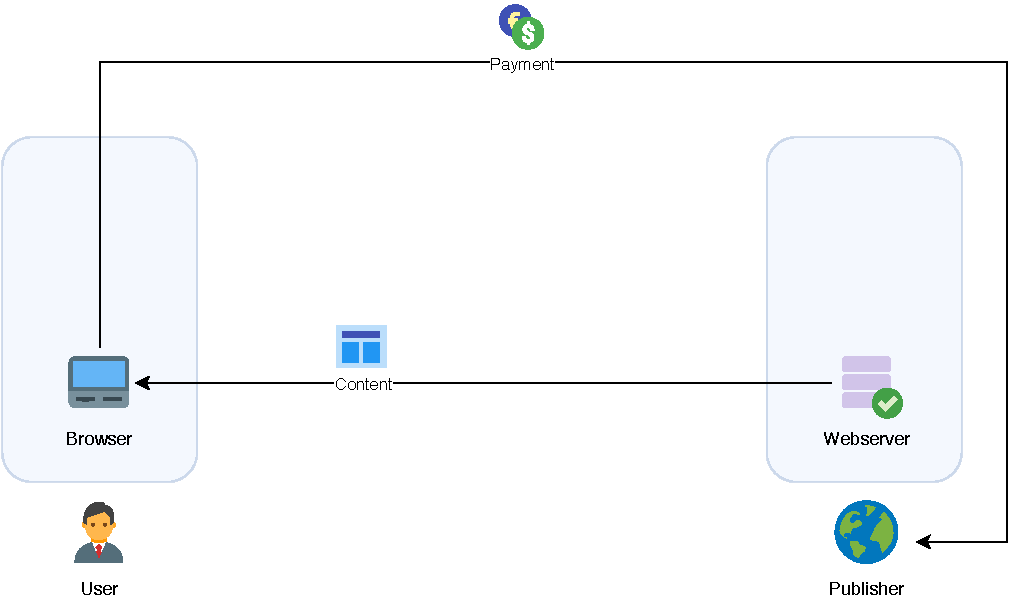
\includegraphics[width=12cm]{images/concept.pdf}
  \caption{Proposed concept overview}
\end{figure}
\vspace{2em}

Concept: \textit{Distribute a small amount of money over the publishers behind the websites you visit and hide the advertisements}

\vspace{2em}

Potential challenges:
\begin{enumerate}
  \item How to keep the configuration as minimal as possible?
  \item What design can be applied to operate the system in a decentralized way?
  \item How to determine the amount of contribution?
  \item How to prevent fraud?
\end{enumerate}


In order to stick to the zeroconf (zero or minimal configuration) principle, the system should work out of the box, without any configuration. To do so, this concept uses WebRTC. WebRTC is a system that enables two browsers to create a peer to peer connection to each other.

This concept assumes that there is a system running that handles all the automated payments to the publisher. The first problem that needs to be solved is: how does the website communicate with the system. Installing an add-on in the browser would violate the zeroconf principle, so this approach uses WebRTC as a message bus. The reason why WebRTC is chosen, is that WebRTC makes it possible for browsers to communicate with each other. Besides, it is also possible for different websites to communicate in the same browser. Normally, this is not so easy because every website runs in a sandboxed environment. For example, if \textit{derspiegel.de} wants to communicate with a system on \textit{example.com}, that is only possible if there is a link between both websites, such as an iframe or if one of the websites opened a tab to the other one. 

WebRTC connects to an IP address, so what happens if it is connected to localhost? Is it possible to let two websites communicate without a link between them? The WebRTC is indeed able to connect to localhost, but in order to do so, a handshake is needed \cite{dutton2013webrtc}. This handshake, however, is not specified in the WebRTC protocol. This means the system can implement its own way of doing so. WebRTC-systems that are applied on the Internet are mostly relying on a signaling server, which forwards the handshake. 

During this research, several experiments are performed using WebRTC. Unfortunately, it turned out that it is not possible to connect two websites within one browser directly. A signaling server that is run by a third party stays neccesary. This would introduce a privacy problem, because the third party would be able to find out which publisher is visited from which IP address. Therefore, considering this thesis, the concept with WebRTC is abandoned at an early stage.

The approach above, however, does not include any form of payment. In the first stage, the scope is limited to a universal payment system, without taking care of the payment itself. It is assumed that there is a cryptocurrency solution that can be attached to the universal payment system.

Fortunately, parallel to this research, a micropayment solution based on the Bitcoin block\-chain is being actively developed. This so-called Lightning Network is discussed in Section \ref{sec:lightning} in more detail. The goal of this system is to provide instant micropayments at minimal costs, which is ideal for an automated payment solution.

From the concept point of view, the payment part is a matter of communicating with an API. Nonetheless, due to some issues with the Lightning Network, it is not yet ready. One of the main disadvantages of the Lightning Network is that it is not possible to send a transaction to an address directly. By design, a payment should be requested by issuing an invoice. The invoice is written according to a standard format and can be paid using any Lightning Network client. This invoice-based structure is suboptimal for the usecase that is needed for this research.

As it was shown, the concept where WebRTC is applied in order to let the publisher communicate with the system, is not viable. Therefore, this research is extended to other approaches. One approach that is used by other websites to communicate with the users' computer is by running a webserver. This webserver can be accessed from any website by connecting to localhost. For example, the popular video conferencing application Zoom uses this approach so that the application gets opened when a user visits a meeting URL \cite{zoomwebserver}.

As this concept is built in combination with the Lighting Network, there needs to be an application running on the users' computer anyway. This makes it possible to develop one service that needs to be installed, which acts like both a Lightning Network client and an interface on localhost to the website that requests a payment.


\section{Wallet address listing}

As described in the Lightning Network concept, there is a possibility to send micropayments to a publisher. The challenge in this case is, how to communicate the wallet address of the publisher to the users' computer? Of course, it is possible to just store it somewhere in a JavaScript variable. A potential security flaw in this approach is that some websites are executing user generated content, for example: it is possible to host a website with JavaScript content on \textit{github.io}. In that case it is not desirable that a fraudulent party spams JavaScript snippets over the Internet that asks for an automated payment without contributing to valueable content. 

One aspect of websites is barely modified by user generated content: DNS records. DNS records are only modifyable by the owner of the domain name, which, in most cases, is the publisher. One way of storing information in DNS records is to just create a subdomain that contains the content: in this case, the wallet address of the publisher. 

Fortunately, the DNS specification also features a so-called TXT record. This is a record that does not affect the way the domain name is resolved. However, it can be queried and used by other applications. For the automated payment design, the TXT record is used by the system to provide the wallet address of the publisher, so that it cannot be modified by someone else, other than the owner of the domain name. 

\section{Self-signed, DV, OV and EV certificates}

One of the problems with an automated payment system is: how can be determined if a publisher is trustworthy? For example: what happens if some malicious publisher buys a bunch of domain names and opens 50 tabs on the users' computer? Does the system make a payment to all 50 domains? 

One approach would be to assign one party that is able to determine which publisher is trustworthy and which one is not. This would violate the decentralized principle of the concept and is therefore not desirable. Another approach that is discussed is to calculate some kind of score, such as pagerank, and use this score to value the credibility of the publisher. Based on this credibility, a payment might be made or might be adjusted. For example: the domain name \textit{spiegel.de} has a pagerank score of 8/10 where \textit{gartenforum.de} has a pagerank score of 3/10. This ranking, however, does not indicate the trustworthyness of a publisher. There is no legitimate reason to pay more to a big publisher than to a small independant content creator. 

Fortunately, there is already a worldwide decentralized system in place that validates credibility of websites: SSL certificates. SSL certificates, that are needed in order to establish an encrypted connection to a website, are also applied to make sure that the user is communicating with the website that it pretends to be. In order to understand this concept, a short introduction to the different types of certificates and architecture is given. 

First, a certificate needs to be issued by an authority. The credibility of the certificate is based on the credibility of the issuer. If some publisher issues the certificate by themselves, it is called a self-signed certificate and this provides no credibility other than that the connection is encrypted. There is no guarantee that the party on the other end of the line is the party they are pretending to be. If the issuer is a trusted party, the certificate is called a certification authority (CA). These CA's are trusted by the browser or SSL library, and they are doing a couple of background checks before they are issuing a certificte. The level of background checks depends on the type of certificate. 

The least secure type of CA certificate is the Domain Validation (DV). These certificates are available for free and can be used by anyone that owns a domain name. Therefore, a DV certificate does not say anything about the credibility of the publisher. A fraudulent party is able to register a bunch of domain names and also apply for certificates.

A more secured certificate is the Organization Validation (OV), also known as a High Assurance certificate. With this type of certificate, the issuer does some background checks in advance. These background checks include the verification of the information in a third party database, such as a companies house. One other aspect of these certificates is that they are not free, which means that it is less easy to register a bunch of domain names. Major publishers, such as \textit{spiegel.de} are using these OV certificates.

As an extension to the OV certificate, there is an Extended Validation certification. In the past, this type of certificate was popular amongs banks and government agencies, because it showed the name of the legal entity in the browser when such a certificate was used. EV certificates are even more expensive, as the background checks are comprehensive.

These aspects of SSL certificates are very valueable in order to determine the credibilty of a publisher. The default setting of the universal payment solution will be that automated payments are only made to publishers with an OV or EV certificate.

\section{Revenue distribution}

One of the challenges of this concept is to pay a fair share to the publisher. How to determine the amount that is contributed? The general idea is that the amount should be in the same order of magnitude as the revenue when an online advertisement is displayed. In online advertisement jargon such a display is called an impression. The price of such an impression is determined as Cost-per-mille (CPM), the price for 1,000 impressions. If a user clicks on an advertisement, the fee is called the cost-per-click (CPC). The amount of users that clicks on the advertisement is expressed in click-through-rate (CTR) \cite{evans2009online}. For the Google Display Network (which also includes services like Gmail), the following average numbers are available for the first quarter of 2018 \cite{cpmgoogle}: 

\begin{itemize}
  \item CPM: 2.80 USD
  \item CPC: 0.75 USD
  \item CTR: 0.35\%
\end{itemize}

\noindent With this data, it is possible to calculate the average revenue per served ad, which is:

\begin{equation}
\cfrac{CPM}{1000} + CTR \times CPC = \cfrac{2.80}{1000} + 0.75 \times 0.0035 = 0.005425 ~\text{USD}
\end{equation}

\noindent In order to estimate the online ad revenue per user per month, this revenue is multiplied with the average amount of ads that are served to a user per month, which is around 1,700 \cite{papadopoulos2018cost}. 

\begin{equation}
  \text{revenue per ad} \times \text{impressions per month} = 0.005425 \times 1,700 = 9.22 ~\text{USD}
\end{equation}
This results in an average revenue per Internet user of 9.22 USD per month. This, however, does not include the margin of the advertising networks, which is somewhere between 20 and 50 percent. For the Google Display Network it is 32 percent \cite{googlefee}. If we subtract this fee from the calculation above, the remaining profit for all publishers is:


\begin{equation}
  \text{revenue per month} \times (\text{1 -- ad network fee}) = 9.22 \times (1 - 0.32) = 6.26 ~\text{USD}
\end{equation}


This net profit per Internet user per month forms the basis for the pricing model of this concept. By using these numbers, there should be no difference between targeted advertising and this concept in terms of revenue for the publisher.

The next question that needs to be answered is: how to distribute this amount over the publishers in a fair manner?  

The simplest way would be to do $\cfrac{c}{n}$, where $c$ is the contribution per month and $n$ is the amount of publishers. The problem with this approach is that this cannot happen on the fly. $n$ is unknown during the visit of the website. One approach would be to just pay all the publishers once at the end of every month, but that would introduce a lot of risk and prevent the system from making contributions in real time. 

Another approach would be to just make an assumption on $n$, and pay out to the publishers accordingly. If $n$ is reached, the payments will stop. This system is still not ideal, because such assumption is hard to make.

The solution that is presented in this concept, uses a hybrid form of both approaches described above. The system will set a budget per day, based on the calculations above. Lets call this budget $b$. If the user visits a website, the contribution to that particular website will be $\frac{1}{10}$ of the budget. For example: lets say the budget is 20 cents per day. The users visits an article on The Guardian, $\frac{1}{10}$ of the budget, which is 2 cents, is sent to the guardian. Afterwards, the users visits a Wikipedia article, $\frac{1}{10}$ of the budget is sent to Wikipedia. However, only 18 cents of the budget is left. Now $\frac{1}{10}$ of 18 cents, which is 1.8 cents, is sent to Wikipedia. As time passes, the budget is topped up every minute by $\cfrac{b}{1440}$.

Using this approach, the user will never overspend the budget $b$, but is still able to contribute to every website that he visits. One concern could be that websites that are visited in the beginning in the browsing session are rewarded better than websites that are visited at the end of the browsing session. Nonetheless, the browsing behavior of every user is different. In the end, these differences might equal out.

One other concern about this approach is the payment is based on pageviews. If a user is browsing 20 different Wikipedia articles, that would result in the same revenue as the same user using a search engine 20 times. Of course, it is possible to limit the contribution to only one contribution per publisher per day. But as this concept tries to be an alternative to online advertising. Online advertising generates revenue based on impressions, which means that spending more time on a website generates more revenue. Therefore, this aspect of the revenue is also implemented in this concept. 

Unfortunately, research on this approach did not result in any terminology or a basic mathematical principle. From now on, this approach will be called fractional contribution. 

\chapter{Implementation}
\label{cha:implementation}

The goal of this thesis is not only to come up with a concept that might work in practice: in order to prove the concept, this research consists out of a working proof on concept. All source code of the proof of concept is released under the MIT licence, including the latex source code of this master thesis\footnote{\url{https://github.com/lightning-sprinkle}}.

\section{Universal automated payment solution}
The proof of concept that is developed is called Lightning Sprinkle. This name comes from two aspects of this system. Firstly, it uses the Lighting Network as a micropayment processor. Most systems related to the Lightning Network are referencing/referring so in their name. Secondly, sprinkle comes from the verb sprinkling, which is used in the fairy tale of Hansel and Gretel by the Brothers Grimm. In this story, Hansel and Gretel are walking away from home and sprinkling breadcrumbs along their path. Just like this, the sprinkle system leaves a trail of small payments along the browsing path.
\begin{figure}[h!]
  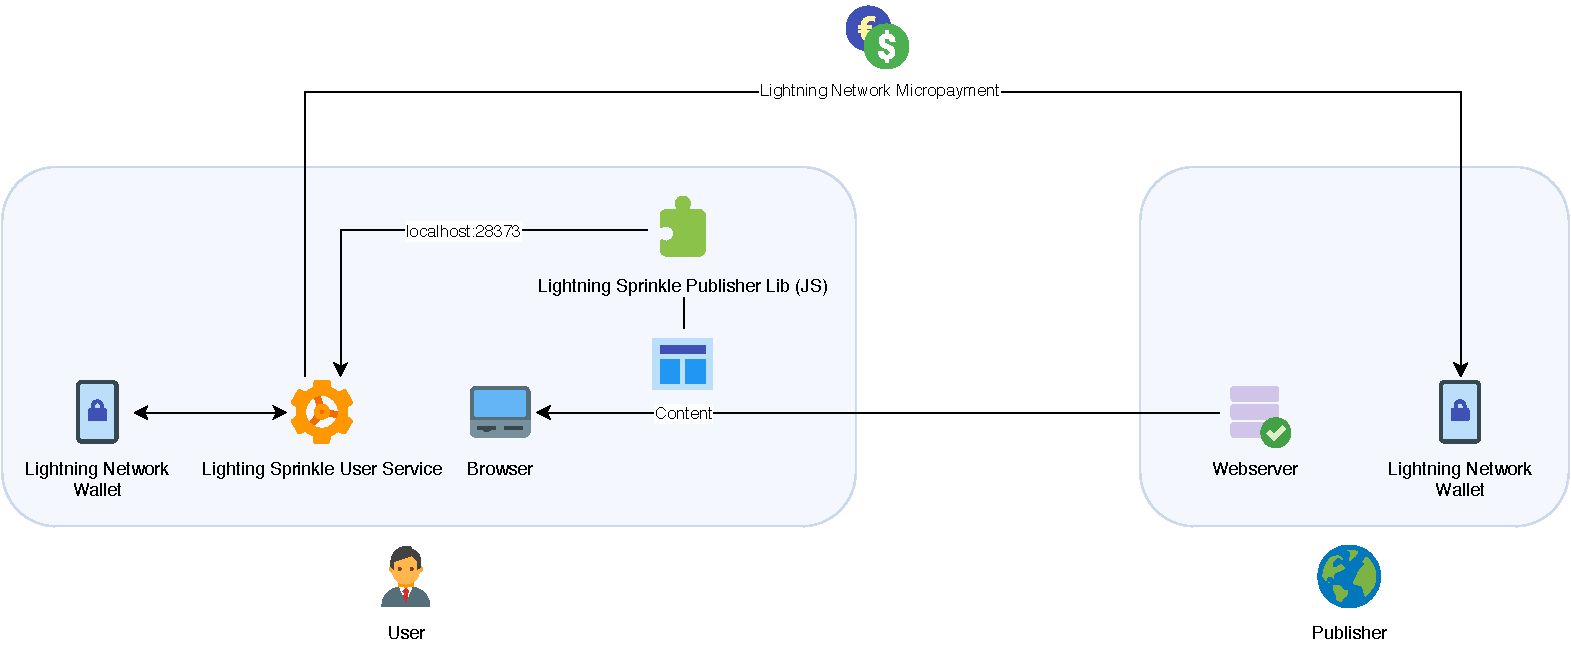
\includegraphics[width=\textwidth]{images/implementation.pdf}
  \caption{Schematic overview}
\end{figure}
In the remainder of this chapter, the following references are used:

\begin{description}
  \item[Lightning Sprinkle User Service] \hfill \\ A service that runs on the users' computer that handles the payments.
  \item[Lightning Sprinkle Publisher Lib] \hfill \\ A Javascript library that is implemented by the publisher in order to request the payment.
\end{description} 

\subsection{Lightning Sprinkle Publisher Library}
According to the concept, as discussed in section \ref{sec:webrtc}, there needs to be a method for the publisher to communicate with a system on the users' computer that handles the payment to the publisher. Normally it is not easy to communicate with services that are running on the users' computer, because this might introduce security flaws as this makes the computer exposed to any script on any website that is visited. The standard way of interaction between the website and other software on the computer is using a browser extension. This, however, adds an extra step in the installation process. Therefore, other ways of interaction are researched.

\subsubsection{WebRTC}

WebRTC enables peer to peer connections between any website or server, which also includes connections between websites and services on one computer. The main idea is that the Publisher Library does some port scanning on the users' computer and connects to the User Service.

During the implementation, it turned out that it is impossible to create a webRTC connection between two instances directly. Compared to traditional TCP connections, it is not possible to connect to an arbitrary port without a proper handshake beforehand. The handshake and discovery process as implemented in the webRTC protocol is called signaling. Normally, this handshake is handled by a signaling server that functions as a handshake broker.

Unfortunately, introducing a central authority that handles the handshakes would disrupt the decental aspect of the entire system. Several alternatives are discussed, such as creating a decentral network of signaling servers, however this would make the situation far more complex for such a small part of the entire ecosystem. Therefore, this approach is abandoned after a few experiments.

\subsubsection{postMessage()}
A different method of passing messages between different websites is the \textit{postMessage} functionality in Javascript. This makes it possible to interact with different websites. In order to use the \textit{postMessage} method, there needs to be a link between both websites. Such a link only exists when one website is opened by another. This happens for example when website A opens website B in a new window or tab. The same link also exists when website B is loaded into an iFrame. 

Using this message system, it is possible for the Publisher Library to communicate with an instance of the User Service. The disadvantage of this approach is that it is limited to the web ecosystem: messages can only be transmitted to other websites, not to services that are running on the users' computer. 

On the basis of advancing insights, during experiments with the Lightning Network, it turned out that it is not feasible to create a system that runs completely inside the web ecosystem. Therefore, this approach is limited to the exploration phase and not implemented in a/the prototype.

\subsubsection{Localhost}
\label{sec:localhost}

The final approach to the problem of connecting from the publisher library to the user service is using localhost. The idea stems from how the videoconferencing tool Zoom connects to their software from an arbitrary website. The principle relies/builds on the fact that it is possible to load content from websites that are hosted on another domain. This also includes localhost.

In practice, any website can connect to any other domain. Examples of application can be found in abundance in/of web tracking. For example, if a user visits a website that uses third party tracking, a request is made to the third party from the users' computer to send data, such as tracking cookies, to the ad network. 

This implementation aims to make it possible for the publisher library to connect to the user service on the local machine in order to request an automated payment. The user service includes a web server that can be accessed by the publisher library. 

The ability to create requests to different domains introduces plenty of security issues. It might leak data that is only intended for the uses/use/users on other domains or even trigger an action on another website. This is known as cross site scripting (XSS) vulnerabilities. Therefore, browsers have taken security measures in order to prevent these undesired side effects.

Firstly, as a website, it is possible to configure the Cross-Origin Resource Sharing (CORS). This parameter can limit the amount of websites that are allowed to send a request to them. Secondly, so-called mixed content is not allowed. This means that if the website runs on https and initiates a request to a third party that is on http, the request is blocked by the browser. Thirdly, Chrome is actively blocking any requests to localhost, as this might expose services that are running on the local machine.

The first security measure can be circumvented easily by setting \\\texttt{Access-Control-Allow-Origin:*}, which means that any publisher using the Publisher Library is able to connect to the User Service. 

The second measure is harder to circumvent. As of 2020, every self-respecting website uses https, so it is not/im-possible to not support the Publisher Library on https websites. /so not supporting the Publisher Library on https websites is not possible. There are a couple of ways to make it still/zonder still possible to support https enabled publishers to connect to localhost:

%twijfel over deze dubbele punt. En daarnaast: de eerste zin hieronder is nogal abrupt: ineens is het probleem opgelost. Twijfel of je daar iets meer woorden aan vuil moet maken.
 
Firstly, the User Service can support https, so that is not an issue anymore. However, in order to support https, there needs to be a certificate that is used to encrypt the traffic to localhost. Such a certificate can only be issued if a domain name is used. With localhost, this is not the case. So, the only option is to generate a self-signed certificate. Self-signed certificates, however, are not trusted by browsers, so requests are still blocked. To support this self-signed certificate, the user needs to make an exception in the browser for this particular certificate. This method is not very user-friendly and violates the zeroconf principle, which makes it suboptimal.

Secondly, there is an exception/ an exception is made (by XXX) for media content that is being loaded from external resources. The standard way of performing requests to another website from Javascript is using an \texttt{XMLHttpRequest}, but these requests are facing limitations like the one described above/like the one on self-signed certificates. However/On the other hand? When a website just embeds an image from another website, there are very little limitations. Fortunately, it is possible to load an image in a programmed way and transfer data using this image.

The implementation of this is quite simple: the Publisher Library loads an image that is located on localhost, for example: \texttt{http://localhost:28373/status}. Then the User Service receives the request and is able to answer with an image. The content of the image is hard to parse/watisdit? in the Publisher Library, but metadata like the dimensions of the image are easy to read. Using this approach, (a) two-way communication is possible between the Publisher Library and the User Service. The User Service responds to the request by sending an image with a particular dimension. In this case, for example, responding with an image that has a width of 2, means that the system is running and the publisher is approved.

\subsubsection{Asking for permission}
As stated in chapter \ref{cha:conceptanddesign}, the system relies on the type of certificate the publisher has. If this certificate is based on organization validation (OV), the system pays to the publisher automatically. For smaller publishers, who cannot afford such a certificate, the Publisher Library can request permission to get paid. 

The system that asks for permission also relies on the web ecosystem. The publisher library checks if this publisher is permitted. If this is not the case, a pop-up window is opened which opens a web page that is hosted on localhost by the user service. The user service is able to find out which publisher made the request by reading the referral header. The user is able to accept the request, which adds the domain name to the whitelist. In the future, this publisher is also able to request automated payments.

\begin{figure}[h!]
  \setlength{\fboxsep}{0pt}%
  \fbox{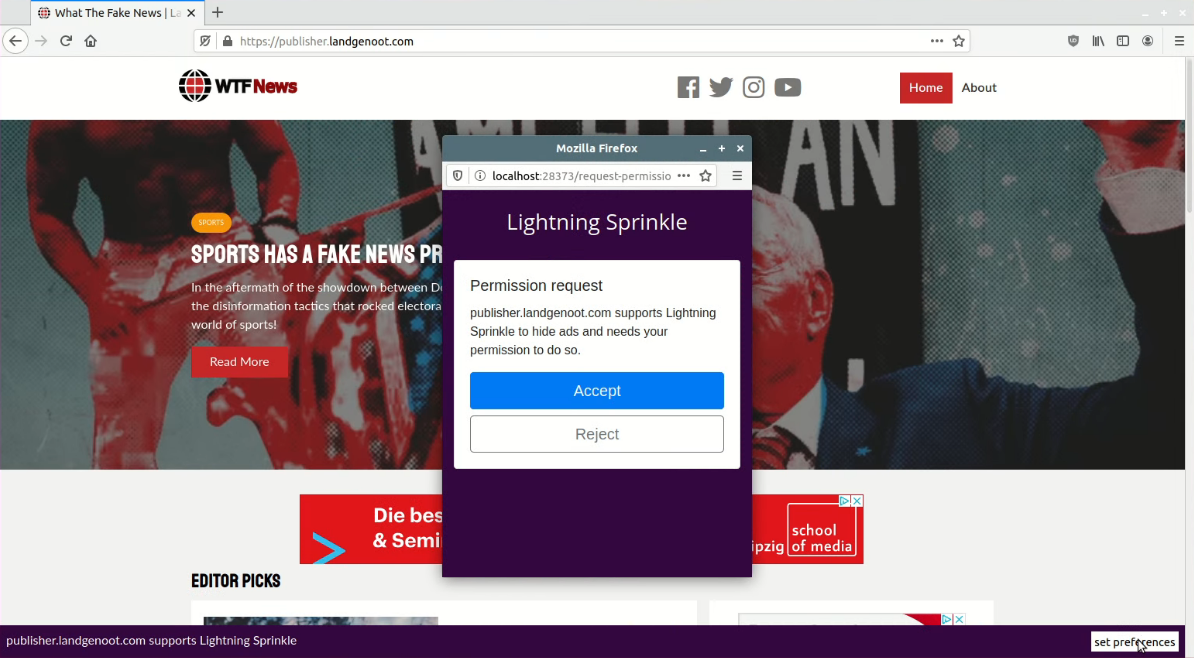
\includegraphics[width=\textwidth-2px]{images/popup.png}}
  \caption{Popup that asks for permission}
\end{figure}

\subsection{Lightning Network}
\label{sec:lightningnetwork}

Now there is an ecosystem that enables publishers to communicate with a service that runs outside the browser. This service, somehow, needs to make a micropayment. As discussed in the chapter \ref{cha:relatedwork}, existing payment service providers are not suitable as it would/since they violate the decentral principle. Therefore, the landscape of cryptocurrencies suitable for micropayments is researched. It turned out that the lightning network is the most promising solution, as it relies on the cryptocurrency with the largest market cap/? and is still able to process instant payments with minimal fees. The principle of the lightning network is already explained in chapter \ref{cha:conceptanddesign}. This section will explain what challenges were faced during the implementation of the proof-of-concept.

The lightning network is not a single implementation. The creators of the lightning network decided to create a request for comments (RFC) instead. This RFC describes how the network should function and by what rules. Several other parties are implementing clients that follow these standards/this standard. However, because of the current work-in-progress state of the system, there are small differences between the clients and even between different versions of clients. 

In order to run a lightning node, which is a client that is part of the network, an application with multiple components is needed. 

Firstly, there is a normal bitcoin client needed, in order to communicate with the bitcoin network and perform transactions on the blockchain. This bitcoin client also takes care of the private keys that are needed to sign any transaction.

Secondly, there needs to be a lightning network node. This client handles all the communication with the lightning network, and also interacts with the bitcoin client in order to open or close channels. 

Thirdly, as/since all (the) transactions that occur over the lightning network are easy to follow, there needs to be some form of obfuscation. Otherwise, it will be easy to link an IP address to a lightning transaction.

%En waarom is dat een probleem?

\begin{figure}[h!]
  \setlength{\fboxsep}{0pt}%
  \center
  \fbox{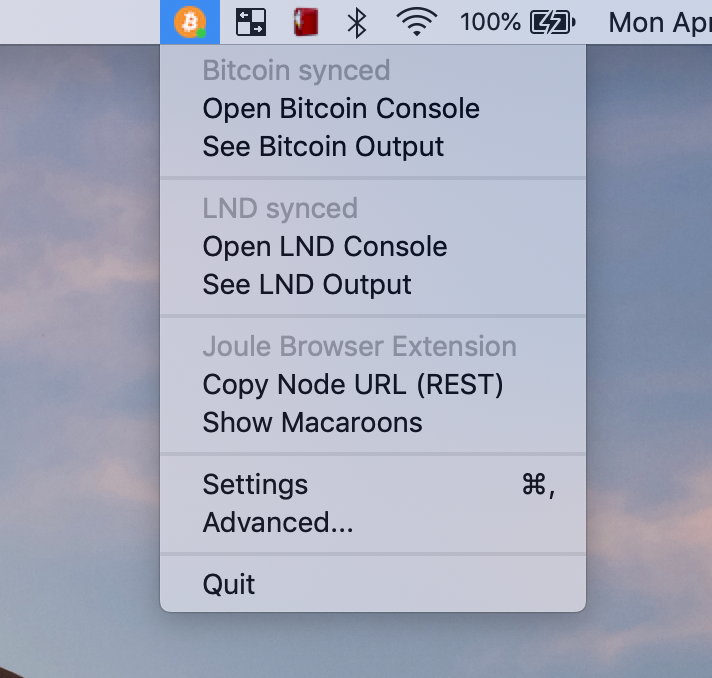
\includegraphics[width=15em]{images/node-launcher.png}}
  \caption{The node-launcher application}
\end{figure}

The node-launcher can be described as package bundle with all the components listed above, written in Python. It takes care that all the components are configured correctly and are up and running. It also features a tray application that shows the status of the application. In the first phase, this application is adopted as a lighting network solution as this application is easily modifiable.

When the node-launcher is running, there is no interface to interact with the lightning network node. It is up to the user to install a front-end that interacts with the lightning node. Examples of these front-ends are the Zap wallet\footnote{\url{https://github.com/LN-Zap/lnd}} or the Joule Browser Extension\footnote{\url{https://github.com/joule-labs/joule-extension}}. For this thesis, however, there is no need for a front-end, as the Lightning Sprinkle User Service is able to interact with then lightning node directly. 

The design of a lightning network transaction is based on a one-time invoice structure. The receiver of the payment needs to create such an invoice first, which will be transmitted in the form of an encoded string or QR-code. This invoice contains details like the amount, payee public key, routing hints and an expiration date. The payor opens this invoice in the lighting network node application, and after that is able to submit the payment.

Due to this structure, it is very hard to make spontaneous payments. When selling products online, this is not an issue/there is no objection against is/..., but for other things than goods and services, this/it is not ideal. This is for example the case with donations. Currently, there are services that offer to create a lightning network donate button that creates a new invoice every time it is accessed. Under the hood, these services are connecting to the lightning network node of the payee and requesting a new invoice every time. For the purpose of this thesis, this is far from ideal, because that means that with every visit of a website/while visiting any website/, multiple other requests are needed in order to exchange the invoice. 

As of 2020, the lightning network is still in an experimental phase and under active development. During the implementation phase of this thesis, the team behind the lnd client explored a way to circumvent the invoice structure\footnote{\url{https://github.com/lightningnetwork/lnd/pull/3795}}. This feature is not yet? part of the official lightning network specification, and therefore also not (yet) widely supported. During the implementation phase of this proof-of-concept, it was only possible to experiment with this circumvention, by using the latest beta (version?) of the lnd client. 

\subsubsection{Keysend}
\label{sec:keysend}

As of 2020, the lightning network is still in an experimental phase and under active development. During the implementation phase of this thesis, the team behind the lnd client explored a way to circumvent the invoice structure\footnote{\url{https://github.com/lightningnetwork/lnd/pull/3795}}. This feature is not part of the official lightning network specification, therefore it is not widely supported. During this implementation phase, it was only possible to experiment with it using the latest beta of the lnd client. 
%eerste keer dat je lnd gebruik (begin paragraaf hierboven). Even uittypen.

The implementation only exists in the latest \texttt{lncli} client. This command line tool connects to the \texttt{lnd} node and is able to interact with it. For example, it can create invoices. If both the payor and the payee are using the latest version of \texttt{lnd} and it is started with the \texttt{--accept-key-send} flag, it is possible to send spontaneous payments using the \texttt{--keysend} flag. It does not matter what configuration, client or version of the lightning network the nodes in between are using. 

Unfortunately, the Lighting Sprinkle User Service needs to connect to the \texttt{lnd} node directly and does not make use of the \texttt{lncli}, therefore it is not a matter of setting the \texttt{--keysend} flag and a deeper understanding of the workaround is needed.

The workaround, however, is not straight forwarded as it seems to be. Normally, the invoice contains a hash of the preimage. The preimage is a cryptographically random bytearray with size 32, that is needed in order to redeem a locked payment. If there is no invoice, we cannot exchange this secret with the payor. To circumvent this issue, \texttt{lnd} makes use of a custom record as part of the payment.

\texttt{KeySendRecord uint64 = 5482373484}

The custom record with this id, contains a preimage that is generated by the payor. Only the payee is payee able to read these custom records and is therefore also able to redeem the payment. The rest of the payment occurs in the standard way.
\lstset{language=Python}
\lstset{frame=lines}
\lstset{caption={Constructing a keysend SendRequest}}
\lstset{label={lst:code_direct}}
\lstset{basicstyle=\footnotesize}
\begin{lstlisting}
def keysend_money(dest, amt):
  """ 
  Transfer money using the experimental keysend method
  """
  # Generate preimage by generating cryptographic safe random bytes
  preimage = secrets.token_bytes(32) 
  payment_hash = hashlib.sha256(preimage).digest()
  # Set the preimage as a custom record in order 
  # to use the experimental keysend method
  dest_custom_records = {5482373484: preimage}

  request = ln.SendRequest(
    dest_string=dest,
    amt=amt,
    final_cltv_delta=40,
    payment_hash=payment_hash,
    dest_custom_records=dest_custom_records
  )
  
  return stub.SendPaymentSync(request, metadata=[('macaroon', macaroon)])

\end{lstlisting}

Interestingly, the custom record functionality is also implemented quite recently. One of the use cases for these custom records are to exchange chat messages over the lightning network (whatsat), so that it acts like a decentral messaging service. 



\subsection{Lightning Sprinkle User Service}

The user service is the component that handles all the requests from the publishers that have implemented the publisher library. In order to do so, an application in Python is built on the Flask framework. This framework makes it easy to create an application in Python that also provides an API.

This application consists out of six modules:
\begin{enumerate}
  \item server
  \item reward
  \item status image
  \item lnd
  \item dns
  \item cert 
\end{enumerate}

Firstly, the server part functions as web server. There are three different API-endpoints: status, request-permission and request-payment. The status endpoint returns whether the origin domain of the request is allowed to request payments. The request-permission endpoint is used to add the origin domain to the whitelist. Lastly, the request-payment endpoint is used to request and execute the automated payment.

Secondly, the reward module keeps track of the budget. Based on a maximal hourly reward, the fee is calculated and used in the micropayments.

Thirdly, the status image module generates an image with given dimensions. This image is used as a workaround in order to support two-way communication, as described in section \ref{sec:localhost}.

Fourthly, the lnd module handles the communication with the lightning network node. This communication is based on gRPC. It provides a function that is able to send a payment to an address immediately using the keysend method. The keysend method is described in more detail in section \ref{sec:keysend}. In order to authenticate at the lnd service, macaroons are used. Macaroons are comparable to cookies and contain authentication data. There are implemented in such a way that different types of macaroon provide different levels of privilege. 

Fifthly, the dns module takes care of the extraction of the DNS entries. As described in chapter \ref{cha:conceptanddesign}, the payment needs to have a destination. Storing the public key of the destination in javascript, introduces potential vulnerabilities as user generated content is able to alter javascript. Therefore, the service relies on TXT-records that are stored at the DNS server. In this way it is guaranteed that the recipient of the payment also controls the DNS records of the domain. This module implements a DNS resolver and looks for a TXT-record that contains a public key according to the following format:

\texttt{lnd-pubkey=027d2456f6d4aaf27873b68b7717b...}

Lastly, the cert module is able to check the credibility of the domain name by looking up the type of certificate that is used. As described in chapter \ref{cha:conceptanddesign}, the presence of an OV or EV certificate indicates enough credibility to automate the payment immediately. 

SSL certificates are structured according to the X509 format. Such/These certificates contains basic info, like the certificate authority and the organization. As the X509 format is designed in 1988, long before they were used for HTTPS, it does not have any option to store the type of certificate directly. In order to differentiate between DV, OV and EV certificates, it/X509 uses a certificate extension called CertificatePolicies. The following policies with corresponding object ids/IDs? are used for the different types of certificates:

\begin{enumerate}[leftmargin=8em]
  \item[2.23.140.1.2.1] Domain Validation
  \item[2.23.140.1.2.2] Organization Validation
  \item[2.23.140.1.1] Extended Validation
\end{enumerate}

By extracting these Certificate Policies, it is possible to determine the type of certificate that a particular domain name uses. 

\subsection{Electron tray application and Neutrino}
The first proof-of-concept, as described in section \ref{sec:lightningnetwork}, uses the normal full \texttt{btcd} daemon. The disadvantage of this method, is that the entire bitcoin blockchain needs to be downloaded. As of 2020, this is over 300GB and takes over 24 hours on an average DSL internet connection. 

However, there are also so-called light wallets available, which/. These wallets/these wallets do not require the entire blockchain to be downloaded. They rely on other nodes and only download the blocks after a certain block number. In order to only download transactions that are relevant for the user(s), bloom filters are used. Bloom filters make sure that a part of all transactions is downloaded that at leat include the transactions of the user. However, because not only the transactions of the user are downloaded, but also some transaction of several other users, the privacy of the user is preserved/guaranteed?

The \texttt{lightning-app}\footnote{\url{https://github.com/lightninglabs/lightning-app}} uses the \texttt{neutrino}\footnote{\url{https://github.com/lightninglabs/neutrino}} light wallet, which makes it much less of a hassle to set up a lightning node. This \texttt{lightning-app} does not require to download the entire blockchain. Moreover, the \texttt{lightning-app} also features an auto pilot mode, where it automatically opens lightning channels, so that the user is able to spend money. This approach makes the proof-of-concept of this thesis much more viable. 

In the second phase of the implementation, two new aspects of this system are introduced: the transition to javascript/electron and the use of the neutrino bitcoin light wallet.

In electron, it is also possible to create a tray application, so that the application keeps running when closed. 


\begin{figure}[h!]
  \setlength{\fboxsep}{0pt}%
  \center
  \fbox{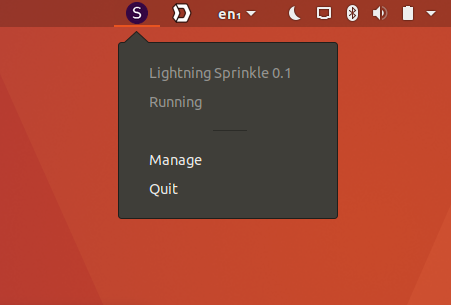
\includegraphics[width=20em]{images/electron-tray.png}}
  \caption{The Lightning Sprinkle Tray Application}
\end{figure}

However, as the thesis is only about developing a proof-of-concept and the translation to javascript/electron took more time than expected, the development of this alternative implementation is not continued.

\subsection{Example website with Google AdSense}
In order to demonstrate the project, a small static website is set up using an open source template. This example website/demo website? shows how a publisher can implement the Lightning Sprinkle Publisher Library. 

To make the example as real life/realistic as possible, the Google AdSense program is joined/added? (if: joined, dan even zin mooi maken), so that Google is able to serve real advertisements on the example website. 

One problem with such (wie? google? even noemen) a third party supplier of advertisements, is that normally there is no toggle to disable the advertisements other than not loading the Javascript library of the advertisement network. Unofficially, however, it is possible to disable advertisements in the same way they are blocked by an Ad Blocker: by removing certain objects from the DOM. For Google AdSense, this is done by the following simple Javascript line:


\lstset{language=Javascript}
\lstset{frame=lines}
\lstset{caption={Disabling Google AdSense advertisements}}
\lstset{label={lst:code_direct}}
\lstset{basicstyle=\footnotesize}
\begin{lstlisting}
  $('.adsbygoogle').remove()
\end{lstlisting}

Using this unsupported/unofficial? method, it becomes possible to let the user decide if he or she either wants to see advertisements or to allow the publisher to request automated payments instead.

The purple bar on the bottom of the example website is placed there/shown/implemented/...? by the Lightning Sprinkle Publisher Library. The button in the bottom (in the bottom klinkt raar. at the bottom? Of heeft de button een bepaald teken?) can be used to add the publisher to the whitelist.

\begin{figure}[h!]
  \setlength{\fboxsep}{0pt}%
  \fbox{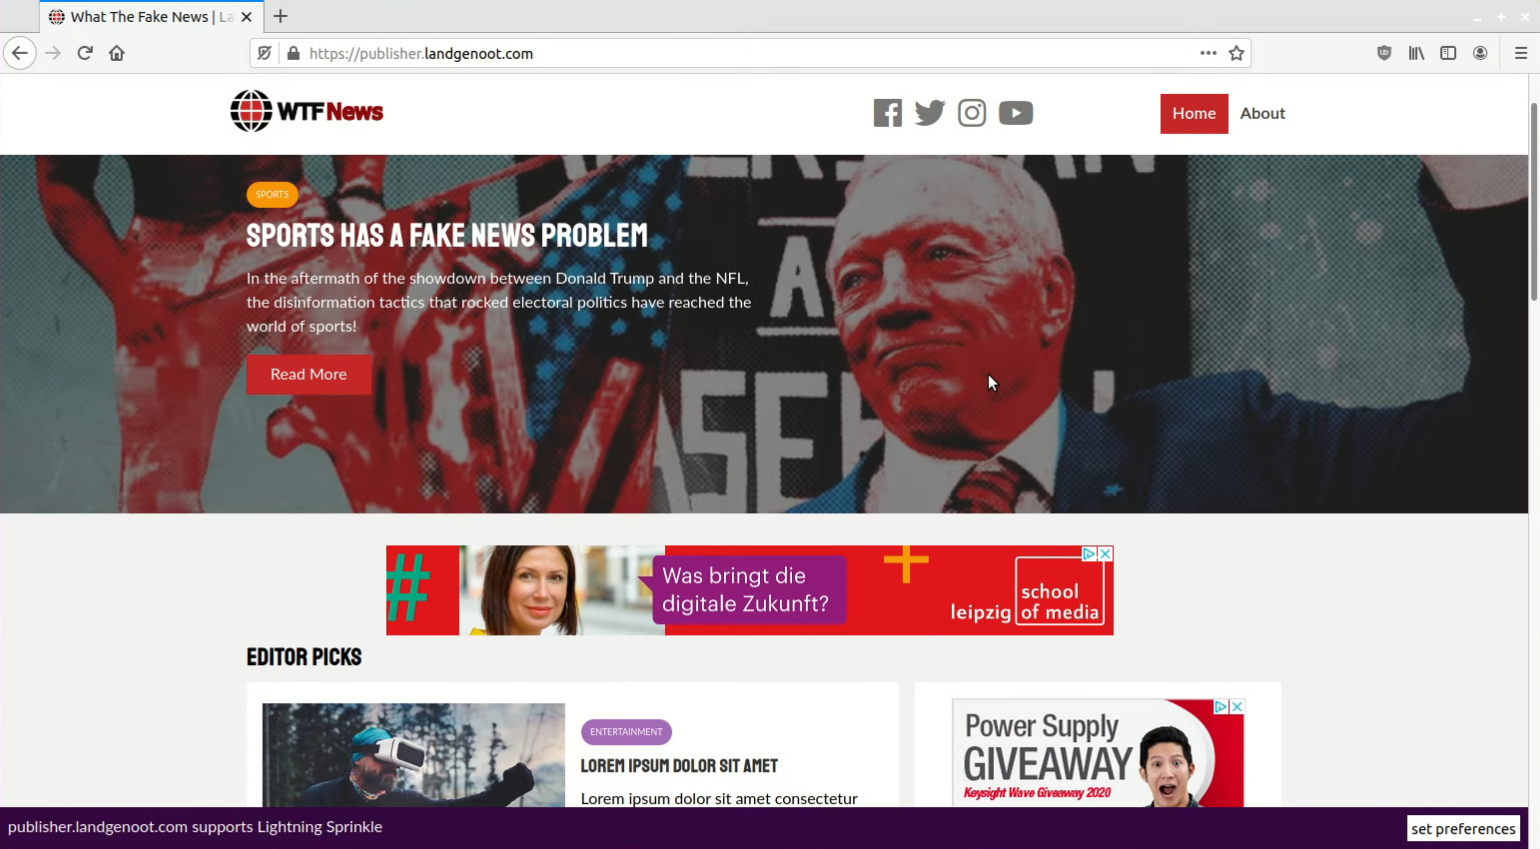
\includegraphics[width=\textwidth-2px]{images/example-website.png}}
  \caption{Example website with ads that implements the Lightning Sprinkle Publisher Library}
\end{figure}

\chapter{Performance Analysis \& Evaluation}
\label{cha:evaluation}

The concept that is designed in this thesis is evaluated with two different software projects: the Lightning Sprinkle User Service and the Lightning Sprinkle Publisher Library, which are written in Python and Javascript respectively. 

The goal of these software projects is to prove that it is possible to implement that is an answer to the concept that is stated in section \ref{sec:uaps}. These requirements will be used as part of the evaluation, combined with a couple of performance tests. Performance tests that include: the scalability of the platform and response time. 

\noindent The original concept from section \ref{sec:uaps} is:

\vspace{1em}

Concept: \textit{Distribute a small amount of money over the publishers behind the websites you visit and hide the advertisements}

\vspace{1em}

\noindent The challenges from the same concpet can be translated into the following requirements:
\begin{enumerate}
  \item Minimal configuration
  \item Decentral
  \item Fair distribution
  \item Tamper proof
\end{enumerate}

Firstly, the minimal configuration requirement can be observed from two perspectives: a world where cryptocurrencies are widely adopted, and the real world. In the first case, the system is just a matter of downloading the application and depositing some money on the bitcoin wallet that comes with the application. After the deposit is confirmed on the blockchain, the rest will go automatically: The application will configure the lightning wallet by opening a channel and will accept requests from publisher that are using the Lightning Sprinkle Publisher Library. 

In the real world, it is not so easy to obtain any cryptocurrency. In most countries, there are laws in order to prevent money laundering and backing of terrorism. For example, in the Netherlands, there is an Anti-Money Laundering and Anti-Terrorist Financing Act\footnote{\url{https://www.toezicht.dnb.nl/en/4/6/51-204766.jsp}}, that requires that any financial institution gathers data about their customers, which also includes cryptocurrency exchanges. The process of converting any fiat currency to a cryptocurrency might consist out of registering somewhere and uploading a copy of an identity document. This makes the whole application more cumbersome and hard to use by non-tech-savvy users. Therefore, the first requirement is met partly because of external limitations.

Secondly, with the decentral requirement, there should not be a single authority that has any power over the network as a whole. This requirement is almost met completely. The system relies on the bitcoin blockchain, which is decentral by design. This also accounts for the lightning network, as this network is also decentral by nature. The only central authorities that the system relies on, are the certificate authorities. A certificate authority might revoke a certificate, so that the Lightning Sprinkle User Service does not send automated payments anymore. However, revoking a certificate results in side effects that are much worse: the browser will reject to connect to the website in first place. 

Thirdly, the fair distribution requirement is hard to satisfy. In first place, there is no existing distribution model that handles this problem. For example, the Brave browser just distributes the money over the publishers and does not take into account things like the frequency of visits are the credibility of the website. This thesis tries to come up with a model that takes frequency of visits into account, but it is still hard to make it really fair. Is a news website that someone visits ten times per day also ten times as valuable as one single Wikipedia article? This topic still has plenty of room for discussion. 

Fourthly, the security of the system in terms of fraud is moderate. The attack where a fraudulent party is able to register a bunch of domain names that all try to request a payment is solved by only allowing domain names with an OV or EV certificate to request a payment immediately. Of course, this is not bullet proof as a party with enough budget is still able to register enough domain names with these expensive certificates. Other attacks might come from malware that is installed on the computer, however, this is in most practical applications of crytocurrencies the case.


\chapter{Conclusion}
\label{cha:conclusion}

Describe what you did here

%--------------------------------------------------------------
% TABLES, FIGURES, BIBLOGRAPHY AND APPENDICES
%--------------------------------------------------------------
\backmatter

% Lists of tables and figures
\listoftables
\listoffigures

% Bibliography
\setwidesite{}						% Set page to be wider for bibliography
\markboth{Bibliography}{bibliography}
\label{cha:bibliography}
\bibliographystyle{IEEEtran}
\bibliography{bibliography.bib}

% Use following to separate online (websites) and offline (books, papers) sources
%\printbibliography[heading=offline,filter=offline]
%\printbibliography[heading=online,filter=online]

\begin{appendices}
	\chapter{Appendix 1}
\label{appendix:listing1}

\lstset{language=PHP}
\begin{lstlisting}
for($i=1; $i<123; $i++)
{
    echo "work harder! ;)";
}
\end{lstlisting}
	% \input{content/99_appendices/a02_listings}
	% \input{content/99_appendices/a03_listings}
\end{appendices}

\end{document}
